\graphicspath{{./design/}}

\chapter{Design}
% {{{
\label{cha:design}

% {{{

The goal of the visualisation aspect of the system is to provide a way to
easily interpret the molecular data. The visualisation techniques chosen either
support the compression aspect of the water compression system, or allow for
general interpretation of data. The main challenge to effective visualisation
of the data is the density of atoms potentially resulting in a cluttered view.

A brief overview of the entire system is provided in Section
\ref{sec:design_overview}, while Section \ref{sec:design_visualisation}
provides more detail of the visualisation components of the system.

% }}}

\section{System overview}
% {{{
\label{sec:design_overview}

The design of the system has been broken down into a number of components. The
most notable components are:

% TODO: more detail
\begin{itemize}
  \item Quantiser - quantises and dequantises the data
  \item I/O - handles input and output of data
  \item Water cluster extractor - extracts the water clusters
  \item Verifiers - verify and record various aspects of the compression system
  \item Arithmetic coders - encodes and decodes symbols
  \item Visualisation - displays the simulation data
  \item Compressors - drivers behind the compression system
\end{itemize}

See Figure \ref{fig:design_overview} for a schematic diagram of the components
listed above. Julian Kenwood has completed the green areas, Keegan Smith has
completed the cyan areas, while Min-Young Wu has completed the red areas. The
Quantiser, I/O and Water cluster extractor components are used by both the
compressors and the visualisation. The Verifiers and Arithmetic coder
components are used by the compressors only.

% TODO: more info
\begin{figure}[h!]
  \begin{center}
    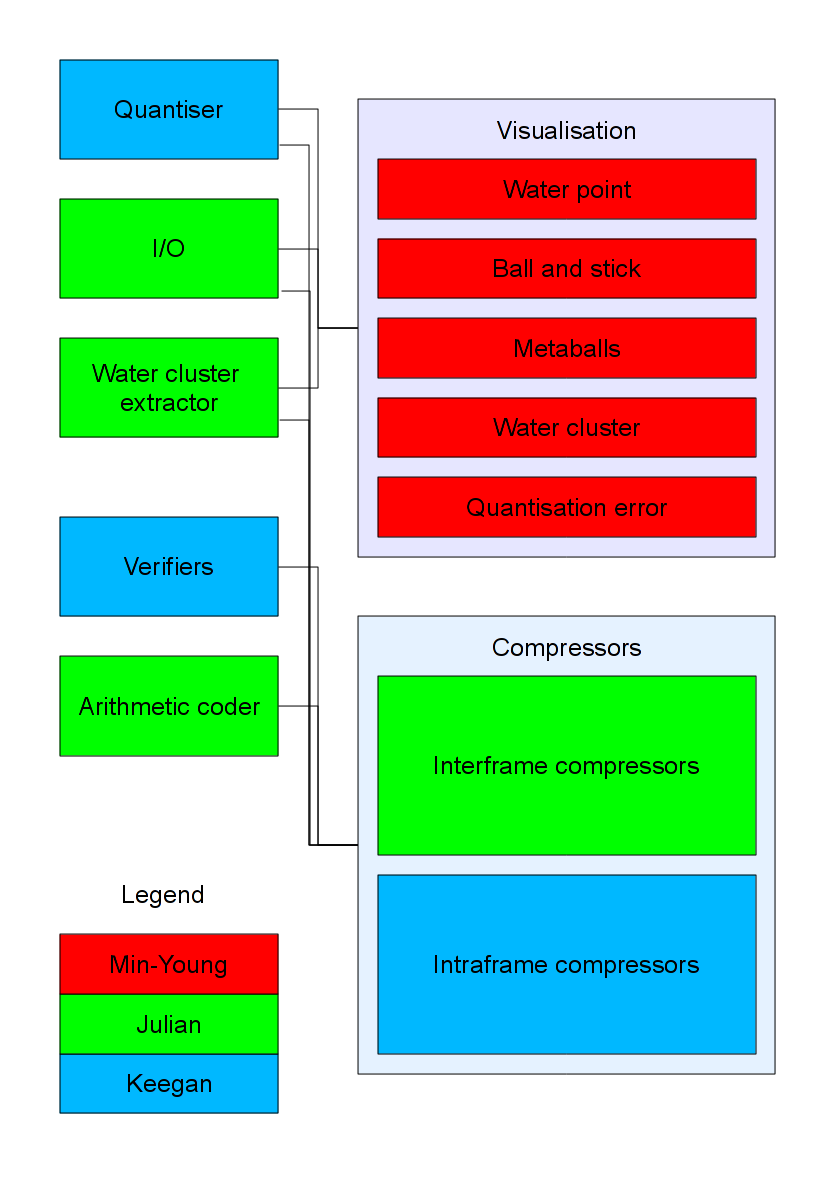
\includegraphics[width=100mm]{breakdown}
  \end{center}
  \caption{Overview of components within the system.}
  \label{fig:design_overview}
\end{figure}

% }}}

\section{Visualisation}
% {{{
\label{sec:design_visualisation}

% {{{

The visualisation component is divided into a number of sub-components, each of
which represents a different visualisation technique:

% TODO: briefly define each
\begin{itemize}
  \item Water point visualisation
  \item Ball-and-Stick visualisation
  \item Metaballs visualisation
  \item Water cluster visualisation
  \item Quantisation error visualisation
\end{itemize}

% }}}

\subsection{Water point visualisation}
% {{{
\label{sub:design_waterpoint}

This visualisation technique is the simplest of all the visualisation
techniques in the system. A single point primitive is rendered per water
molecule, with non-water molecules being filtered out. Filtering out the
non-water molecules is the first step in reducing visible clutter. Using a low
alpha value per point further reduces clutter by causing areas with few
overlapping points to appear more faintly, in comparison to areas with many
overlapping points; hence emphasising the latter areas.

The advantage of this visualisation technique is that it allows for the regions
of high water density to be easily identified, however, the details are hidden.

% }}}

\subsection{Ball-and-stick visualisation}
% {{{
\label{sub:design_ballstick}

% TODO: define ball-and-stick
The ball-and-stick visualisation technique is used to provide more visual
information about the water molecules, with the individual atoms of water
molecules being visible. Rendering the individual atoms allows for the
orientation of the water molecules to be seen.

% TODO: how reduce number of molecules
As rendering all the water molecules will cause significant clutter, the number
of molecules to render can be limited.

% }}}

\subsection{Metaballs visualisation}
% {{{
\label{sub:design_metaballs}

% TODO: define metaballs
The metaballs technique is an alternative way to visualise the water volume in
the molecular simulation. The aim of the metaballs technique is to clearly
separate the areas of water, from the non-water areas. A surface is rendered
between the water and non-water areas of the volume.

To decrease the rendering costs, the surface is decimated. Decimating the
surface will decrease the number of surface primitives, hence decreasing time
required to render it, and allowing the volume to be more easily explored.

An alternative to decimating the surface in order to decrease the surface
complexity, is to decrease the level of sampling. Sampling the volume less
densely results in fewer triangles, but the surface quality will also decrease.

% TODO: how is surface quality maintained
Decimation is preferred over reduced sampling as the surface quality can be
maintained. The render cost is decreased in exchange for computation cost,
where the computation is performed once for every frame, but can be done as a
pre-process.

% }}}

\subsection{Water cluster visualisation}
% {{{
\label{sub:design_watercluster}

The water molecules in a body of water do not group uniformly in all
directions, instead the water molecules form clusters. The compressors use this
knowledge to perform prediction, and thus it is useful to visualise these water
clusters.

% TODO: fix fix fix
To cope with the large number of water clusters that are present, the number of
clusters to render can be limited. Specific water clusters can also be rendered.

% TODO: support less use with reference
This visualisation technique is primarily useful in supporting the compression
aspect of the system. There has been little emphasis on water clusters in
chemistry, thus it is unlikely that this visualisation technique will be of
interest to chemists.

% }}}

\subsection{Quantisation error visualisation}
% {{{
\label{sub:design_quanterror}

% TODO: uhm, something to do
Quantisation is the only lossy step in the compression, thus it is important to
measure the amount of error that is introduced. To visually depict the
quantisation errors, the water molecules are coloured according to a colour
gradient. Water molecules with high quantisation errors are coloured so that
they are more visible and stand out, while water molecules with low
quantisation errors will be less visible.

This visualisation technique is only useful in supporting the compression aspect
of the system.

% }}}

% }}}

\section{Summary}
% {{{
\label{sec:design_summary}

TODO

% }}}

% }}}

